\section{Introduction}\label{sec:intro}

A rational cohomology class on a smooth complex projective variety is a
\emph{Hodge class} if it has type $(p,p)$, and it is \emph{algebraic} if it
is a rational combination of classes of subvarieties. Algebraic classes are
Hodge classes, and Hodge asked whether the converse holds \cite{Hod52}. For
divisors it does, by the theorem of Lefschetz on classes of type $(1,1)$
\cite{Lef24}; in general it is open.

Let $X^{n}_{M}\subseteq\PP^{n+1}$ be the Fermat variety
$x_{0}^{M}+\dots+x_{n+1}^{M}=0$. The group $\mu_{M}^{n+2}$ acts on it, its
primitive cohomology splits into lines indexed by characters of this group,
and the Hodge classes are spanned by the lines whose characters satisfy a
balancing condition \cite{Shi79}. Fermat varieties are the varieties on which
the Hodge conjecture has been tested most closely. It is known for
$X^{n}_{M}$ in every dimension when $M$ is prime or $M=4$
\cite{Ran80,Shi79}, when $M\le20$ \cite{Shi79}, and when $M$ is a power of a
prime \cite{Aok87}. Aoki reduced the conjecture for all Fermat varieties of
degree $M$ to finitely many classes, one for each divisor of $M$ that is a
product of an even number of distinct elements of $\{4,3,5,7,11,\dots\}$,
and proved it for the degrees $2^{a}3^{b}5^{c}7^{d}$ with $c=0$ or $d=0$ and
for $2p^{e}$ \cite{Aok83,Aok00}. Peterson added the degrees
$2^{a}3^{b}5^{c}7^{d}$ not divisible by $420$ \cite{Pet26}, and the first
author the degrees $2^{a}3^{b}11^{c}$, $2^{a}3^{b}13^{c}$, and
$2^{a}3^{b}17^{c}$, $2^{a}3^{b}19^{c}$ with $a\le1$ \cite{BBe84hc}. For
fourfolds more is known: da Silva treated the degrees up to
$100$ \cite{daS21},\footnote{The second arXiv version of \cite{daS21}
states, as its Theorem~3.3, the Hodge conjecture for $X^{4}_{M}$ for every
$M$ prime to $6$, but its proof treats only the classes in tensor products
$V(\beta)\otimes V(\gamma)$ of two Hodge lines of lower dimension; the
published version keeps the bound $M\le100$.} Jumagulov the odd degrees up
to $199$ \cite{Jum26}, a computer census of Jumagulov the even degrees up to
$250$ other than $110$, $114$, $220$ and $228$ \cite{Jum26b}, and
\cite[Theorem~B]{BBe84hc} every odd degree.

\begin{maintheorem}\label{thm:main}
Let $M\ge1$ be an integer that is not divisible by $110$. Then every Hodge
class on the Fermat fourfold $X^{4}_{M}$ is algebraic.\footnote{Kang claimed
this for all degrees \cite[Corollary~3.2]{Kan16}, but his proof has a gap. It
bounds a refined motivic dimension of $X^{1}_{M}\times X^{3}_{M}$ through
\cite[Proposition~2.2(iv)]{Kan15}, whose proof writes the level filtration of
a tensor product as $F^{m}(H\otimes H')=\bigoplus_{t+s=m}F^{t}H\otimes
F^{s}H'$, where $F^{p}$ is the largest rational sub-Hodge structure contained
in the $p$-th step of the Hodge filtration. This already fails for
$H=H'=H^{1}(E,\QQ)$, $E$ an elliptic curve, and $m=1$: the K\"unneth
component of the diagonal of $E\times E$ is a nonzero rational class of type
$(1,1)$ in $H^{1}(E)\otimes H^{1}(E)$, so it lies in $F^{1}(H\otimes H')$,
while $F^{1}H^{1}(E)=0$ and the right-hand side vanishes. The preprint
\cite{MMRV26} relies on the same statement for the degrees $33$, $39$ and
$57$.}
\end{maintheorem}

The degrees not divisible by $110$ that the results above leave open begin
with $228=4\cdot3\cdot19$, $258=2\cdot3\cdot43$, $260=4\cdot5\cdot13$ and
$266=2\cdot7\cdot19$. The degree $110$ is an
exception of the method. At that level Aoki's reduction leaves one class, the
image of his class at level $55$, and the induction leaves sextuples that it
cannot lower; we do not know whether their lines are algebraic, and the
theorem says nothing about $X^{4}_{M}$ when $110\mid M$ (\Cref{rem:110}).

\begin{figure}[t]
\centering
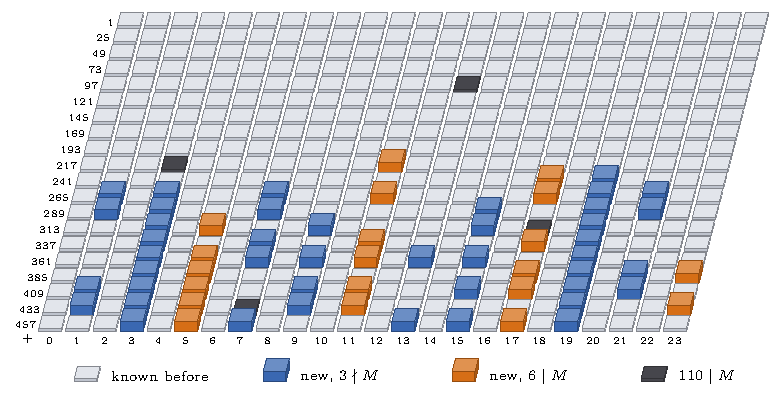
\includegraphics[width=\textwidth]{figures/fig_degrees}
\caption{The degrees $M\le480$, in rows of $24$: the row label plus the
column number is $M$. Light tiles are degrees covered by the results quoted
above, raised tiles are the degrees added by \Cref{thm:main}, and the dark
tiles are the multiples of $110$.}\label{fig:degrees}
\end{figure}

\subsection*{The method}
A Hodge line of $X^{4}_{M}$ is given by a \emph{sextuple}: six nonzero
residues modulo $M$, up to order, that are balanced in the sense of
\Cref{sec:fermat}. Three kinds of sextuples are known to give algebraic
lines: those that contain a pair $\{y,-y\}$, through the inductive structure
of Shioda and Katsura \cite{SK79}; the sextuples that split into two triples
with sum zero, through a product of two Fermat curves; and the standard
multisets of Aoki, through his explicit cycles \cite{Aok87}. A balanced
multiset that meets a standard multiset can be traded for the rest of it, and
we call such a trade a \emph{move}. The proof is an induction on the level and
on the orders of the entries: every sextuple without a pair has a chain of
moves to at most four elements, to a sextuple of smaller orders or to a split
sextuple, or it lies in one of finitely many explicit families, whose lines
we show to be algebraic directly.

The engine of the induction is a linear relation. If the largest order of an
entry of a sextuple $A$ is $e$, the balancing condition, read through Dirichlet
characters of conductor dividing $e$, says that the function counting the
entries of order $e$ in each residue class is a sum of functions that are
invariant under the subgroups $K_{p}$ of units congruent to $1$ modulo $e/p$,
one for each prime $p\mid e$ (\Cref{sec:primetosix}). Such \emph{split}
functions are rigid: a split function of small total mass is supported on a
single coset of one $K_{p}$, and a coset of $K_{p}$ is exactly what a move
needs. The only input from analytic number theory is the nonvanishing of the generalised
Bernoulli numbers $B_{1,\chi}$ for odd characters $\chi$.

\Cref{sec:fermat} recalls the description of the Hodge lines and the
algebraic tools, and \Cref{sec:primetosix} proves the rigidity of split
functions. \Cref{sec:odd} treats odd degrees. \Cref{sec:aoki} sets up Aoki's
reduction, and \Cref{sec:classes} supplies the classes it leaves at the
levels $33$, $35$, $39$, $44$, $52$, $102$ and $114$, by showing that the
relevant parts of the cohomology of Fermat threefolds are supported on
divisors. \Cref{sec:even,sec:four} treat even degrees prime to $3$, according
to the power of $2$ in the largest order of an entry, and \Cref{sec:six} the
degrees divisible by $6$. \Cref{sec:proof} assembles the proof.
